% 2-15-rb-tree.tex

%%%%%%%%%%%%%%%%%%%%
\documentclass[a4paper, justified]{tufte-handout}

% hw-preamble.tex

% geometry for A4 paper
% See https://tex.stackexchange.com/a/119912/23098
\geometry{
  left=20.0mm,
  top=20.0mm,
  bottom=20.0mm,
  textwidth=130mm, % main text block
  marginparsep=5.0mm, % gutter between main text block and margin notes
  marginparwidth=50.0mm % width of margin notes
}

% for colors
\usepackage{xcolor} % usage: \color{red}{text}
% predefined colors
\newcommand{\red}[1]{\textcolor{red}{#1}} % usage: \red{text}
\newcommand{\blue}[1]{\textcolor{blue}{#1}}
\newcommand{\teal}[1]{\textcolor{teal}{#1}}

\usepackage{todonotes}

% heading
\usepackage{sectsty}
\setcounter{secnumdepth}{2}
\allsectionsfont{\centering\huge\rmfamily}

% for Chinese
\usepackage{xeCJK}
\usepackage{zhnumber}
\setCJKmainfont[BoldFont=FandolSong-Bold.otf]{FandolSong-Regular.otf}

% for fonts
\usepackage{fontspec}
\newcommand{\song}{\CJKfamily{song}} 
\newcommand{\kai}{\CJKfamily{kai}} 

% To fix the ``MakeTextLowerCase'' bug:
% See https://github.com/Tufte-LaTeX/tufte-latex/issues/64#issuecomment-78572017
% Set up the spacing using fontspec features
\renewcommand\allcapsspacing[1]{{\addfontfeature{LetterSpace=15}#1}}
\renewcommand\smallcapsspacing[1]{{\addfontfeature{LetterSpace=10}#1}}

% for url
\usepackage{hyperref}
\hypersetup{colorlinks = true, 
  linkcolor = teal,
  urlcolor  = teal,
  citecolor = blue,
  anchorcolor = blue}

\newcommand{\me}[4]{
    \author{
      {\bfseries 姓名:}\underline{#1}\hspace{2em}
      {\bfseries 学号:}\underline{#2}\hspace{2em}\\[10pt]
      {\bfseries 评分:}\underline{#3\hspace{3em}}\hspace{2em}
      {\bfseries 评阅:}\underline{#4\hspace{3em}}
  }
}

% Please ALWAYS Keep This.
\newcommand{\noplagiarism}{
  \begin{center}
    \fbox{\begin{tabular}{@{}c@{}}
      请独立完成作业,不得抄袭。\\
      若得到他人帮助, 请致谢。\\
      若参考了其它资料,请给出引用。\\
      鼓励讨论,但需独立书写解题过程。
    \end{tabular}}
  \end{center}
}

\newcommand{\goal}[1]{
  \begin{center}{\fcolorbox{blue}{yellow!60}{\parbox{0.50\textwidth}{\large 
    \begin{itemize}
      \item 体会``思维的乐趣''
      \item 初步了解递归与数学归纳法 
      \item 初步接触算法概念与问题下界概念
    \end{itemize}}}}
  \end{center}
}

% Each hw consists of four parts:
\newcommand{\beginrequired}{\hspace{5em}\section{作业 (必做部分)}}
\newcommand{\beginoptional}{\section{作业 (选做部分)}}
\newcommand{\beginot}{\section{Open Topics}}
\newcommand{\begincorrection}{\section{订正}}
\newcommand{\beginfb}{\section{反馈}}

% for math
\usepackage{amsmath, mathtools, amsfonts, amssymb}
\newcommand{\set}[1]{\{#1\}}

% define theorem-like environments
\usepackage[amsmath, thmmarks]{ntheorem}

\theoremstyle{break}
\theorempreskip{2.0\topsep}
\theorembodyfont{\song}
\theoremseparator{}
\newtheorem{problem}{题目}[subsection]
\renewcommand{\theproblem}{\arabic{problem}}
\newtheorem{ot}{Open Topics}

\theorempreskip{3.0\topsep}
\theoremheaderfont{\kai\bfseries}
\theoremseparator{:}
\theorempostwork{\bigskip\hrule}
\newtheorem*{solution}{解答}
\theorempostwork{\bigskip\hrule}
\newtheorem*{revision}{订正}

\theoremstyle{plain}
\newtheorem*{cause}{错因分析}
\newtheorem*{remark}{注}

\theoremstyle{break}
\theorempostwork{\bigskip\hrule}
\theoremsymbol{\ensuremath{\Box}}
\newtheorem*{proof}{证明}

% \newcommand{\ot}{\blue{\bf [OT]}}

% for figs
\renewcommand\figurename{图}
\renewcommand\tablename{表}

% for fig without caption: #1: width/size; #2: fig file
\newcommand{\fig}[2]{
  \begin{figure}[htbp]
    \centering
    \includegraphics[#1]{#2}
  \end{figure}
}
% for fig with caption: #1: width/size; #2: fig file; #3: caption
\newcommand{\figcap}[3]{
  \begin{figure}[htbp]
    \centering
    \includegraphics[#1]{#2}
    \caption{#3}
  \end{figure}
}
% for fig with both caption and label: #1: width/size; #2: fig file; #3: caption; #4: label
\newcommand{\figcaplbl}[4]{
  \begin{figure}[htbp]
    \centering
    \includegraphics[#1]{#2}
    \caption{#3}
    \label{#4}
  \end{figure}
}
% for margin fig without caption: #1: width/size; #2: fig file
\newcommand{\mfig}[2]{
  \begin{marginfigure}
    \centering
    \includegraphics[#1]{#2}
  \end{marginfigure}
}
% for margin fig with caption: #1: width/size; #2: fig file; #3: caption
\newcommand{\mfigcap}[3]{
  \begin{marginfigure}
    \centering
    \includegraphics[#1]{#2}
    \caption{#3}
  \end{marginfigure}
}

\usepackage{fancyvrb}

% for algorithms
\usepackage[]{algorithm}
\usepackage[]{algpseudocode} % noend
% See [Adjust the indentation whithin the algorithmicx-package when a line is broken](https://tex.stackexchange.com/a/68540/23098)
\newcommand{\algparbox}[1]{\parbox[t]{\dimexpr\linewidth-\algorithmicindent}{#1\strut}}
\newcommand{\hStatex}[0]{\vspace{5pt}}
\makeatletter
\newlength{\trianglerightwidth}
\settowidth{\trianglerightwidth}{$\triangleright$~}
\algnewcommand{\LineComment}[1]{\Statex \hskip\ALG@thistlm \(\triangleright\) #1}
\algnewcommand{\LineCommentCont}[1]{\Statex \hskip\ALG@thistlm%
  \parbox[t]{\dimexpr\linewidth-\ALG@thistlm}{\hangindent=\trianglerightwidth \hangafter=1 \strut$\triangleright$ #1\strut}}
\makeatother

% for footnote/marginnote
% see https://tex.stackexchange.com/a/133265/23098
\usepackage{tikz}
\newcommand{\circled}[1]{%
  \tikz[baseline=(char.base)]
  \node [draw, circle, inner sep = 0.5pt, font = \tiny, minimum size = 8pt] (char) {#1};
}
\renewcommand\thefootnote{\protect\circled{\arabic{footnote}}} % feel free to modify this file
%%%%%%%%%%%%%%%%%%%%
\title{第3-4讲: 图的基本概念}
\me{林凡琪}{211240042}{}{}
\date{\zhtoday} % or like 2019年9月13日
%%%%%%%%%%%%%%%%%%%%
\begin{document}
\maketitle
%%%%%%%%%%%%%%%%%%%%
\noplagiarism % always keep this line
%%%%%%%%%%%%%%%%%%%%
\begin{abstract}
	% \begin{center}{\fcolorbox{blue}{yellow!60}{\parbox{0.65\textwidth}{\large 
	%   \begin{itemize}
	%     \item 
	%   \end{itemize}}}}
	% \end{center}
\end{abstract}
%%%%%%%%%%%%%%%%%%%%
\beginrequired

%%%%%%%%%%%%%%%
\begin{problem}[CZ 1.2]
仿照例1.1, 自己用9名编辑和8个委员会构造一个例子,并画出相应的图。
\end{problem}

\begin{solution}
	例子:一家大型的出版公司在科学、技术和计算领域内有9名编辑(分别用1,2,...,9)来标记,他们分成8个委员会$c_1 = \{3,4\}, c_2 = \{1,3,5\}, c_3 = \{2,4,6,7\}, c_4 =\{1,3,8,9\},c_5=\{6,7,9\},c_6=\{3,4,8\},c_7=\{1,5\},c_8=\{1,9\}$,这八个委员会在同一天的不同四个时间段内开会.
	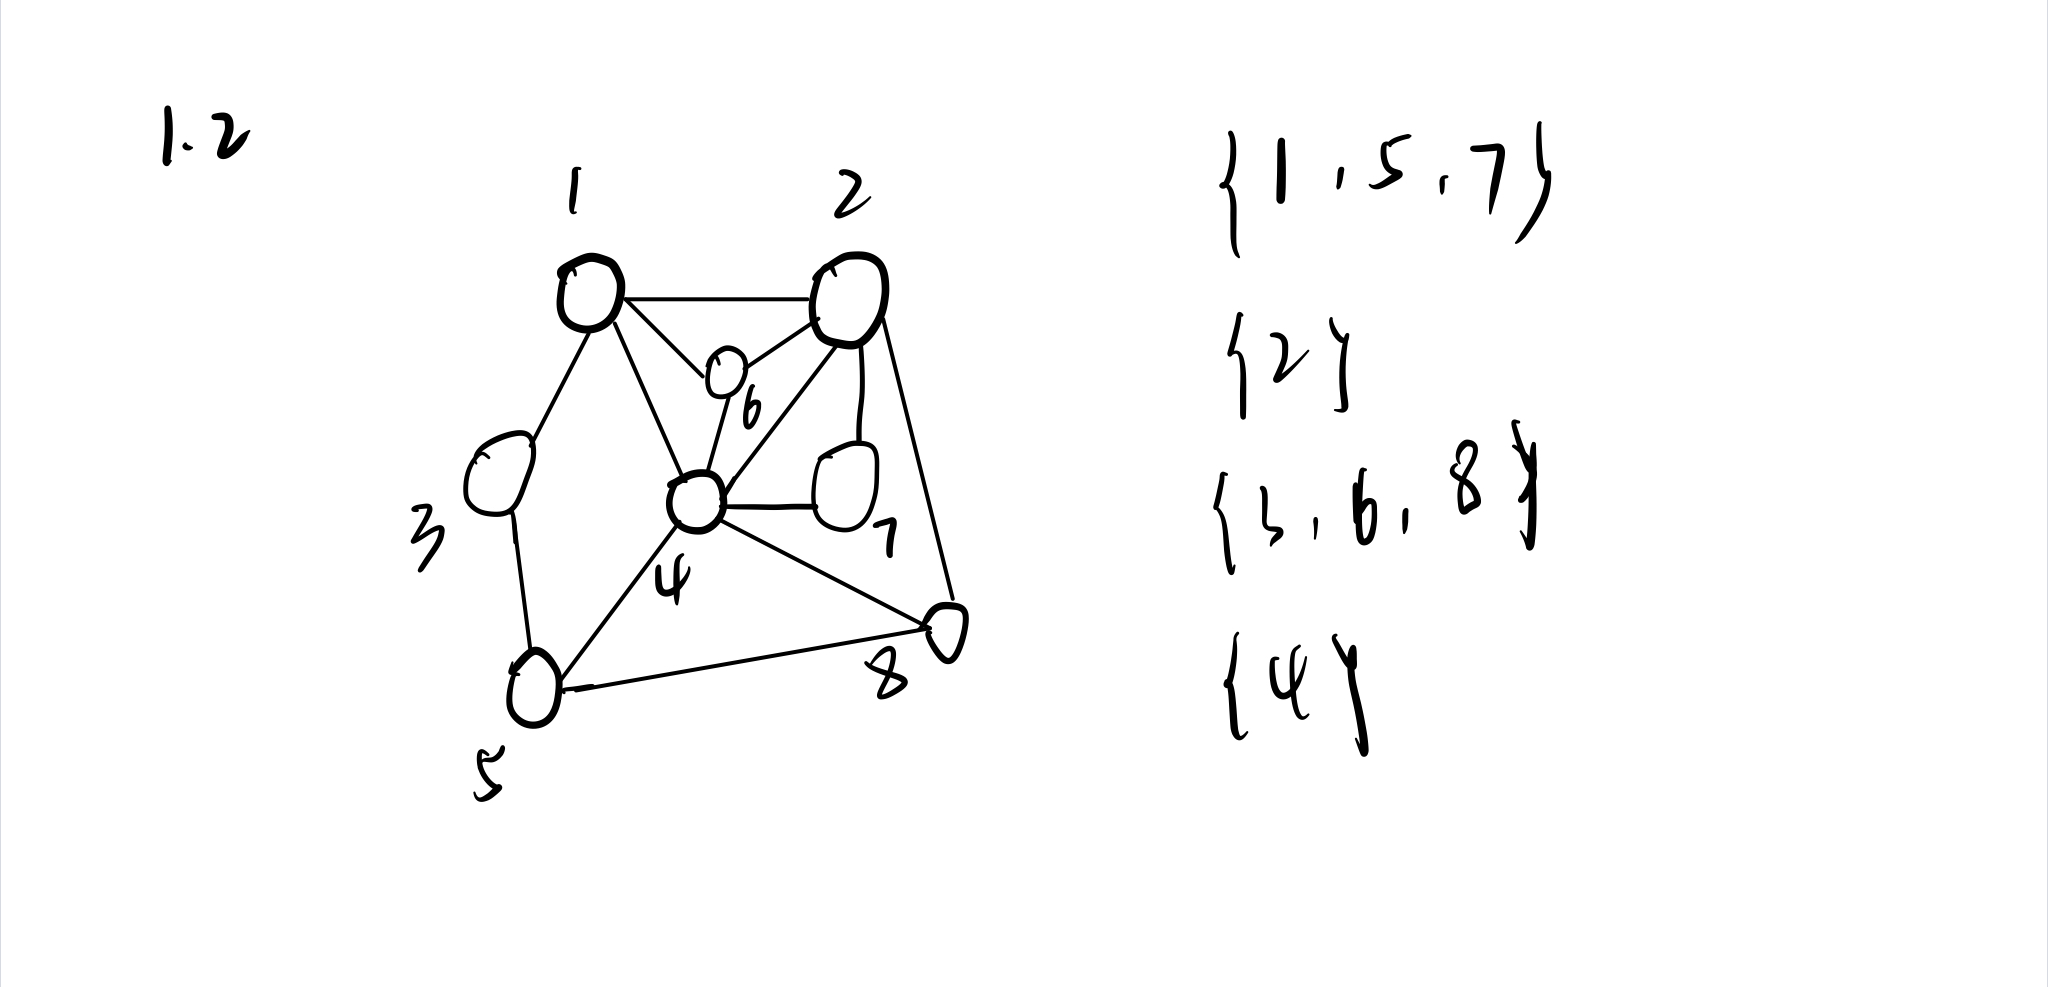
\includegraphics[width = 0.8\textwidth]{1.2.jpg}
\end{solution}
%%%%%%%%%%%%%%%

%%%%%%%%%%%%%%%
\begin{problem}[CZ 1.3]
设$S = \{2,3,4,7,11,13\}$,画出一个图$G$,其顶点集是S,而且对于$i,j\in S$,当$i+j\in S$或者$|i-j|\in S$,则$ij\in E(G)$.
\end{problem}

\begin{solution}
	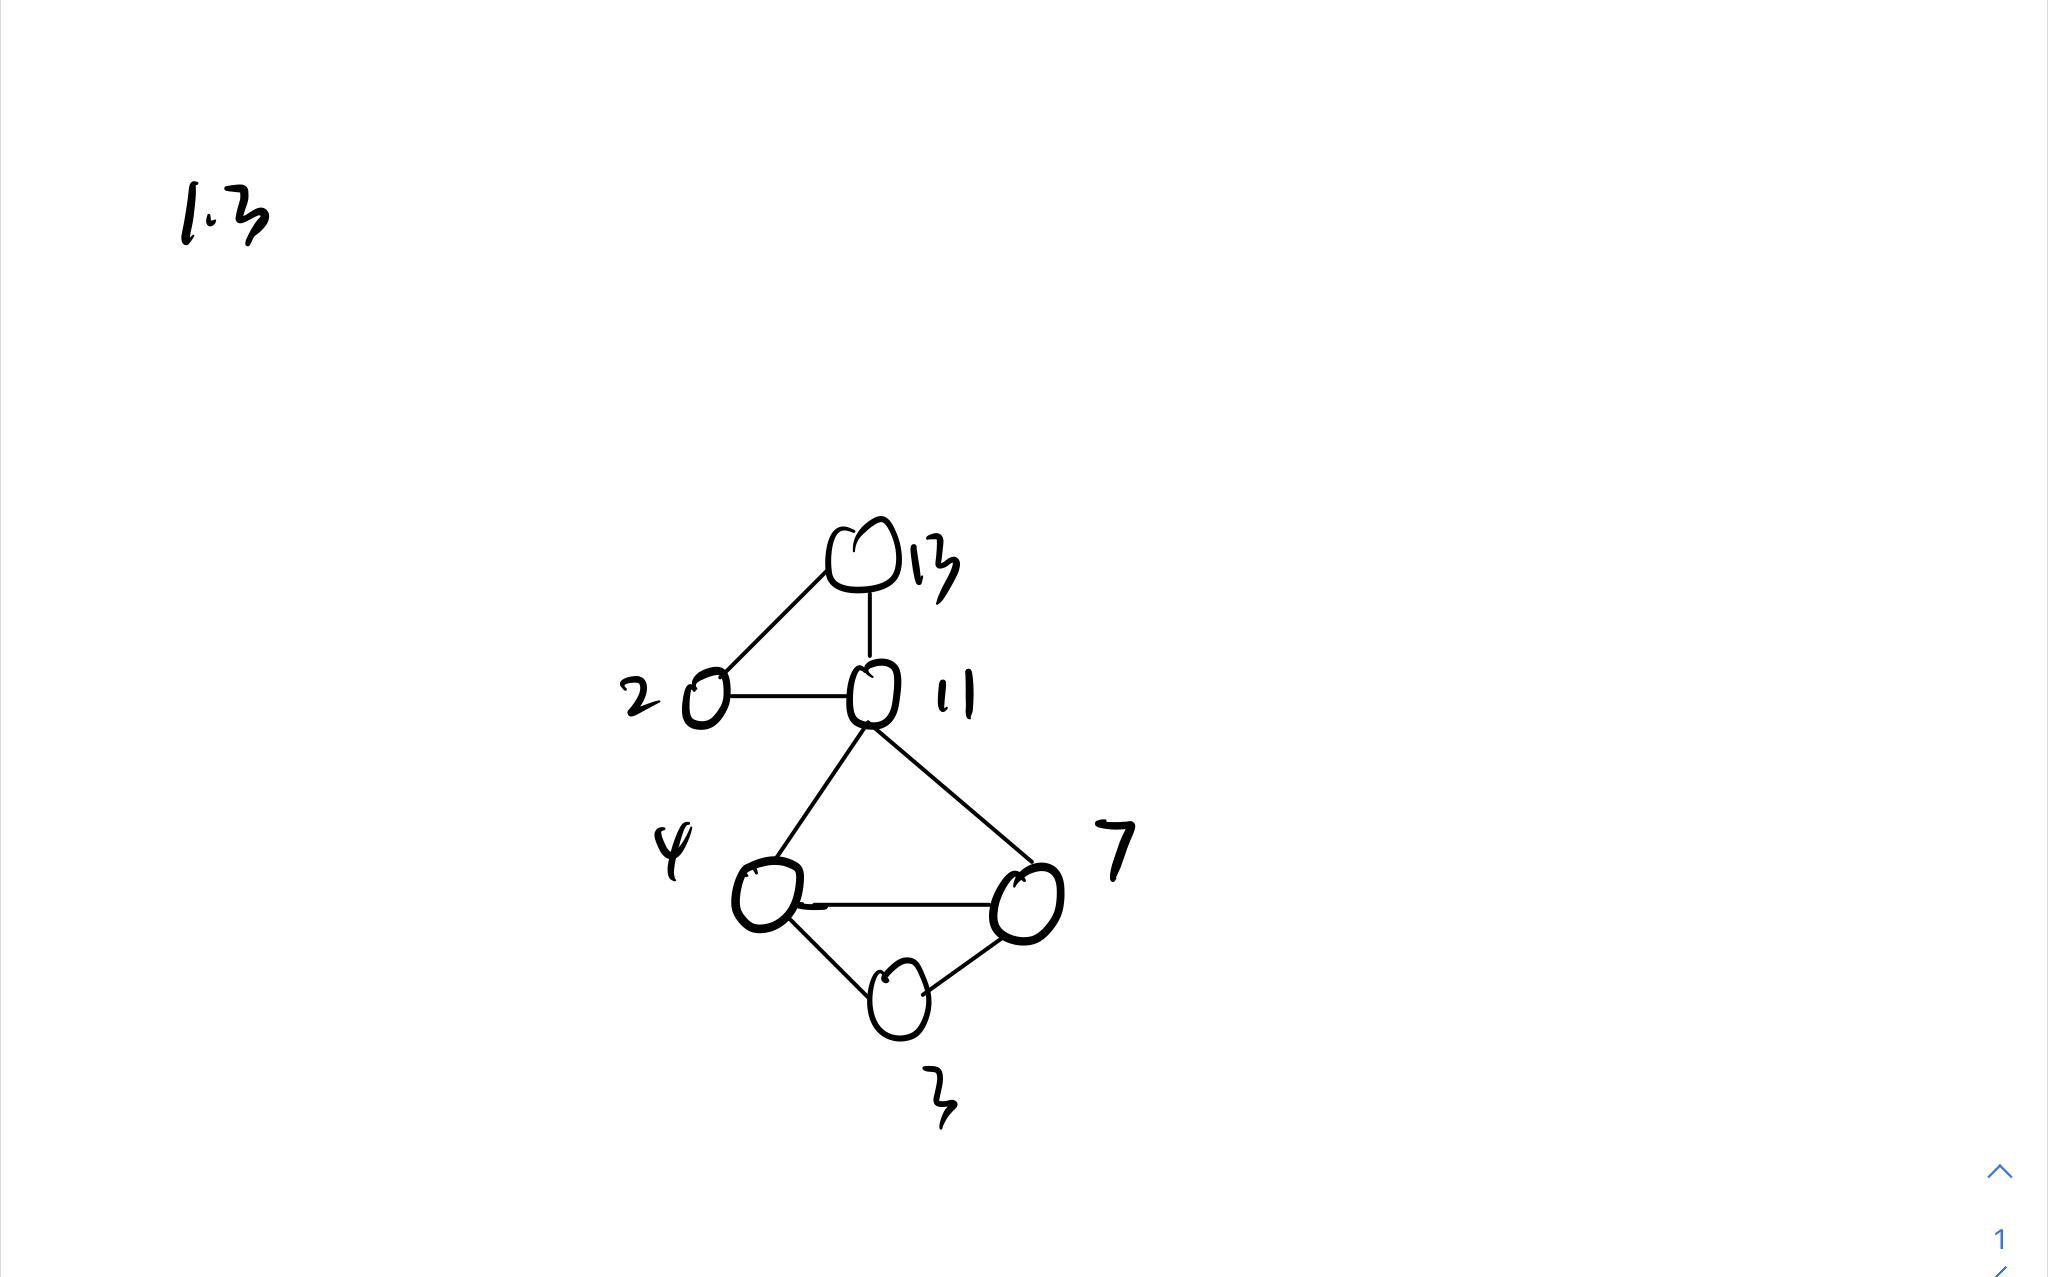
\includegraphics[width = 0.8\textwidth]{1.3.jpg}
\end{solution}
%%%%%%%%%%%%%%%

%%%%%%%%%%%%%%%
\begin{problem}[CZ 1.11]
\end{problem}

\begin{solution}
	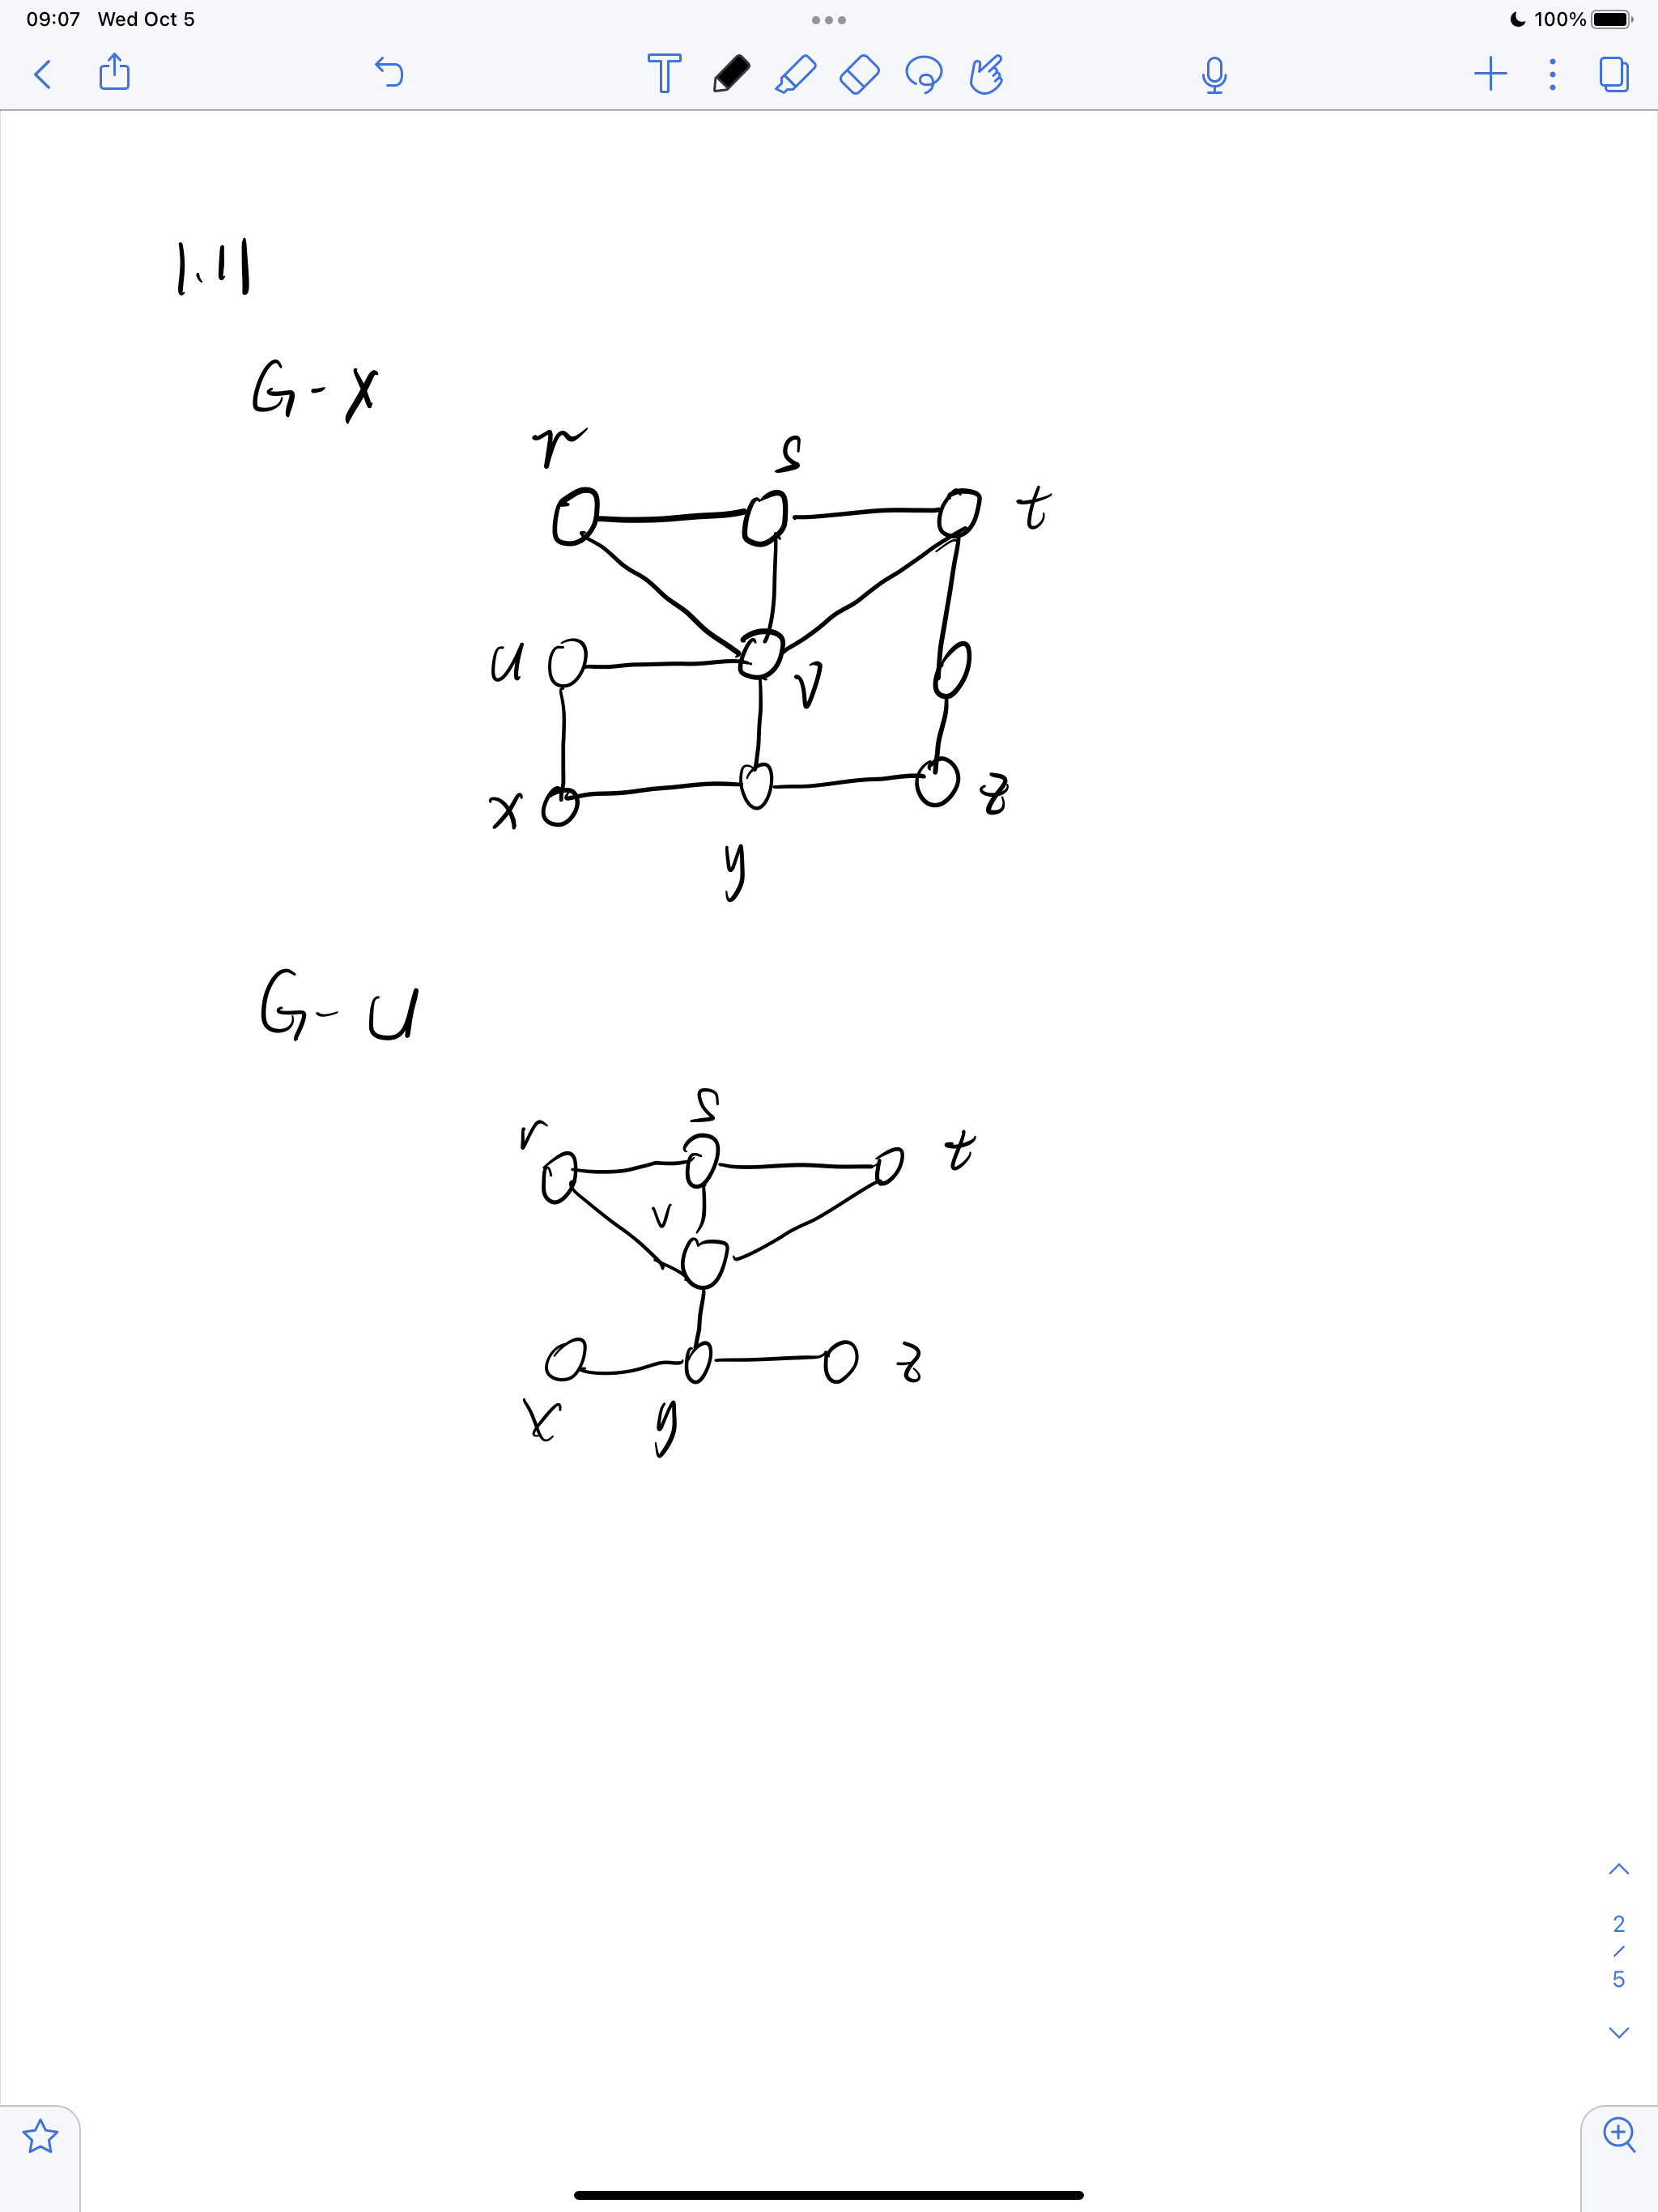
\includegraphics[width = 0.8\textwidth]{1.11.png}
\end{solution}
%%%%%%%%%%%%%%%

%%%%%%%%%%%%%%%
\begin{problem}[CZ 1.12]
\end{problem}

\begin{solution}
	(a)W:x,u,r,v,u,v,y\\
	(b)W:v,u,r,v,w\\
	(c)不存在,r到z最少经过3条边\\
	(d)不存在\\
	(e)W:x,u,v,t\\
	(f)W:r,s,t,v,w,z,y,x,u,v,r\\
	(g)W:r,s,t,v,w,z,y,v,r\\
	(h)W:r,v,y,z
\end{solution}
%%%%%%%%%%%%%%%

%%%%%%%%%%%%%%%
\begin{problem}[CZ 1.24]
\end{problem}

\begin{solution}
	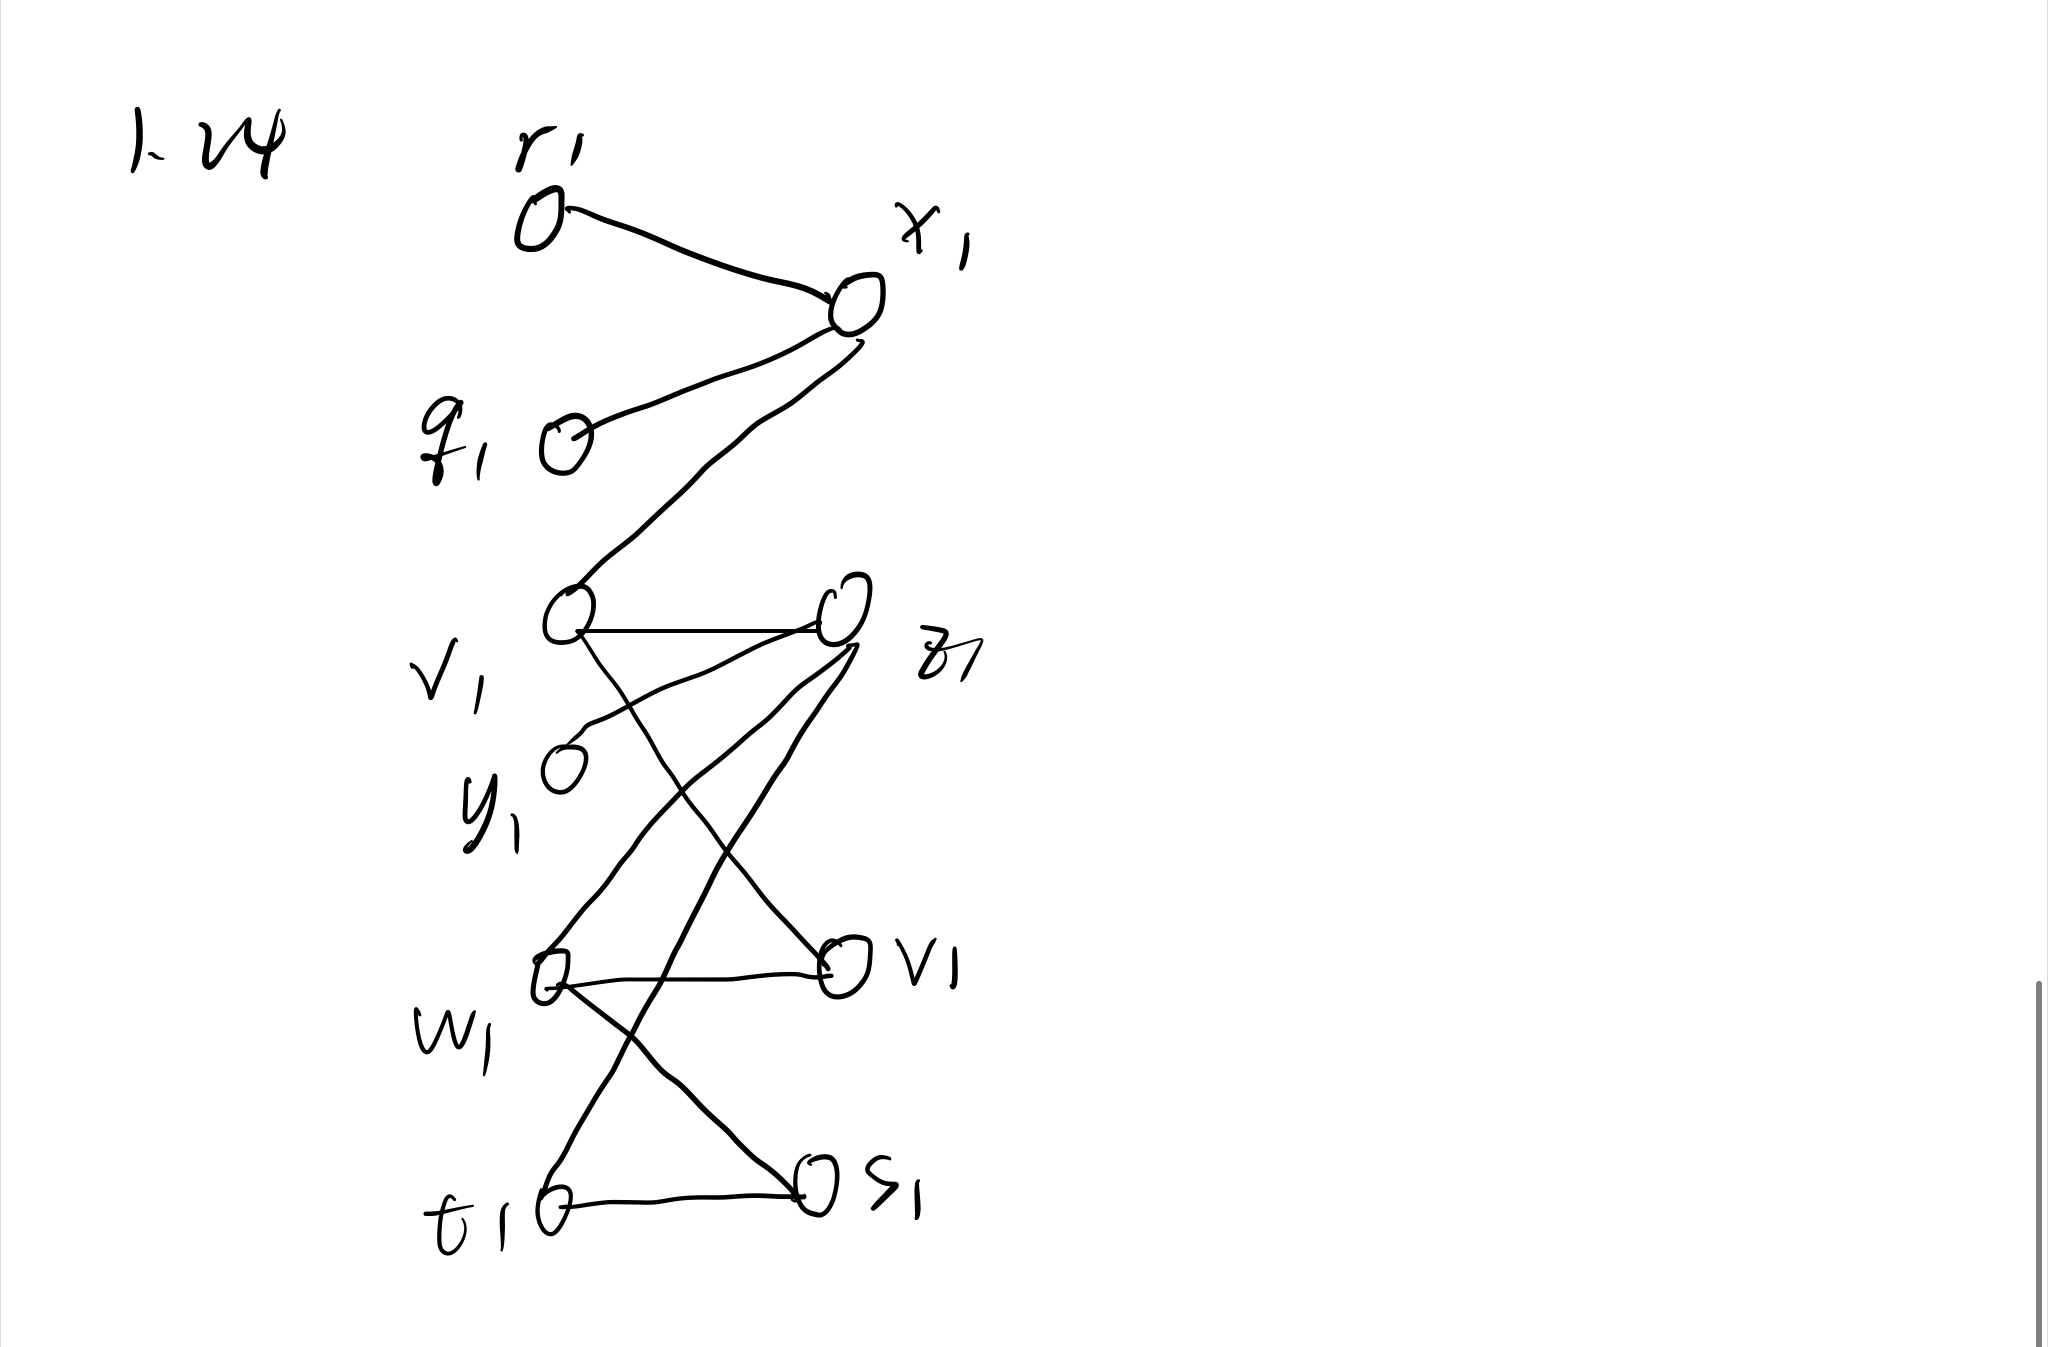
\includegraphics[width = 0.8\textwidth]{1.24.jpg}
	对于第二张图不为二分图,因为其存在奇圈${x_2,r_2,w_2,z_2,y_2}$
\end{solution}
%%%%%%%%%%%%%%%

%%%%%%%%%%%%%%%
\begin{problem}[CZ 2.1]
\end{problem}

\begin{solution}
	(a)不存在。其总度和位13,不为偶数,与图论第一定律相悖。\\
	(b)不存在。点数位7的图,度数最大为6.

	(c)不存在。点数为4的图中度数为3,说明其中有3个点与另外所有点都有连边,则不可能出现度数为1的点
\end{solution}
%%%%%%%%%%%%%%%

%%%%%%%%%%%%%%%
\begin{problem}[CZ 2.19]
\end{problem}

\begin{solution}
	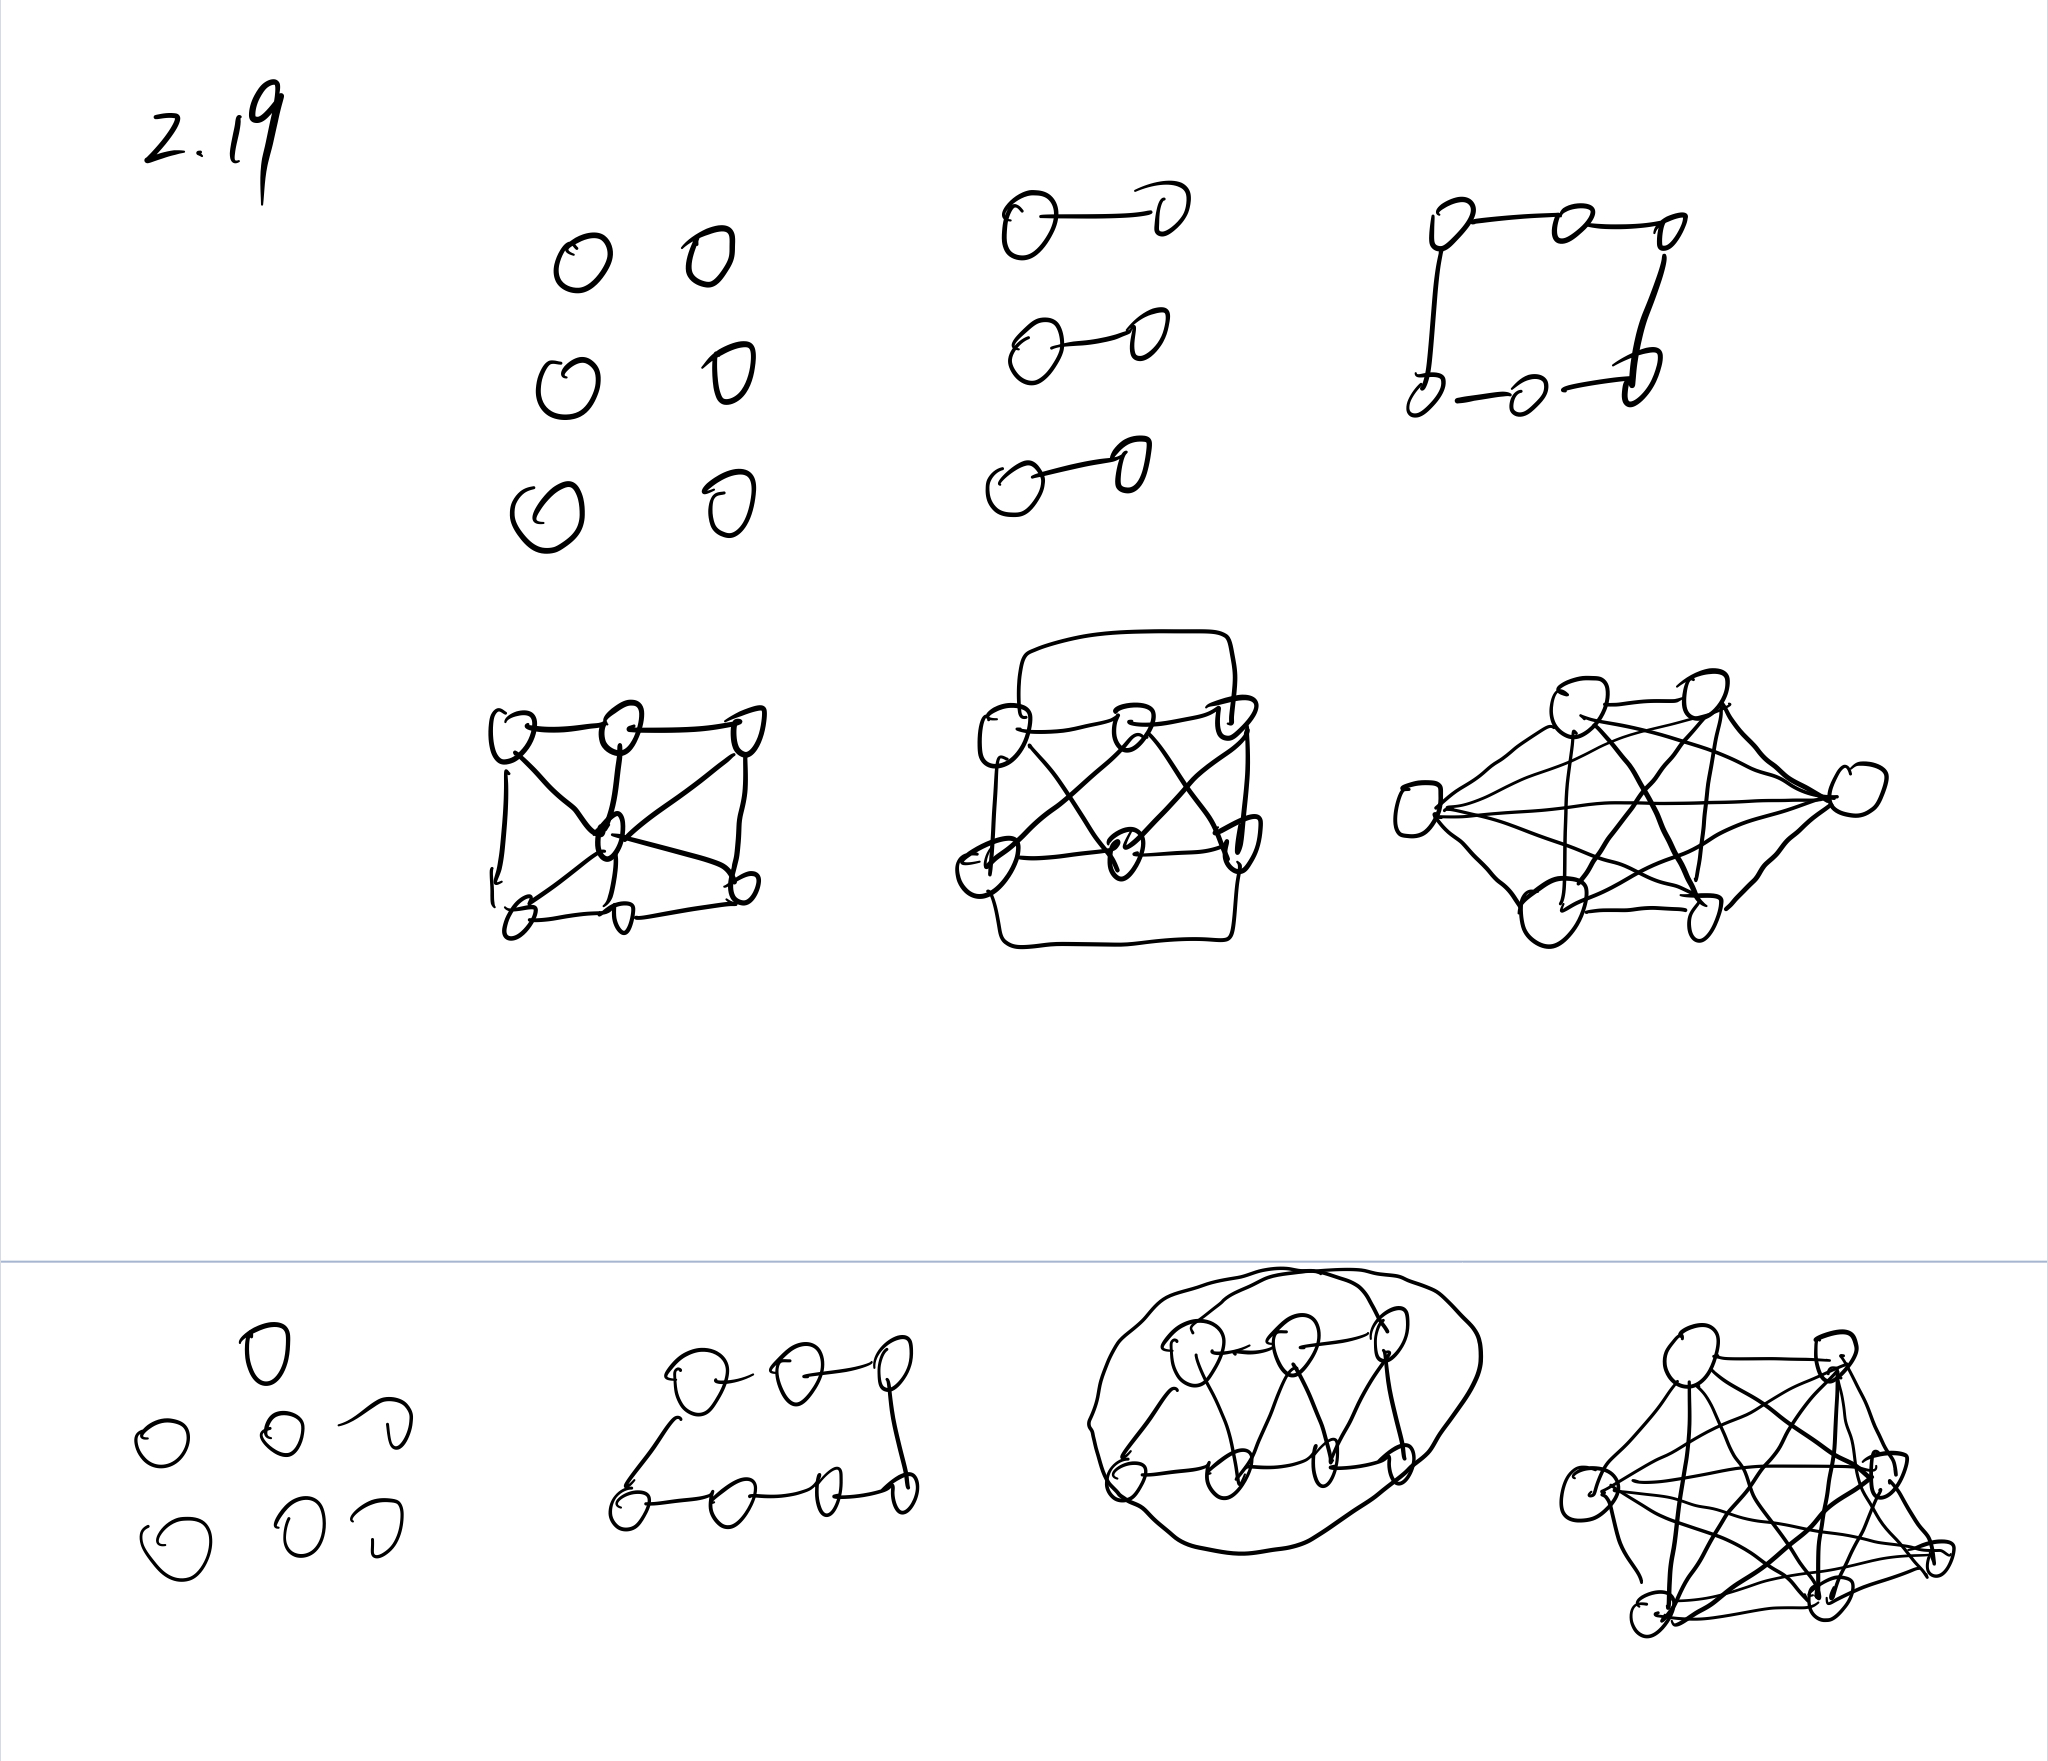
\includegraphics[width = 0.8\textwidth]{2.19.jpg}
\end{solution}
%%%%%%%%%%%%%%%


%%%%%%%%%%%%%%%
\begin{problem}[CZ 2.31]
\end{problem}

\begin{solution}
	假设存在G,度序列为$d_1,..,d_n$,则对其补图,原图G 中度为$d_i$的点,在补图中度为$n-d_i-1$,因此补图存在$n-d_1-1,...,n-d_n-1$的度序列,可图。反之亦成立。
\end{solution}
%%%%%%%%%%%%%%%

%%%%%%%%%%%%%%%
\begin{problem}[CZ 3.1]
\end{problem}

\begin{solution}
	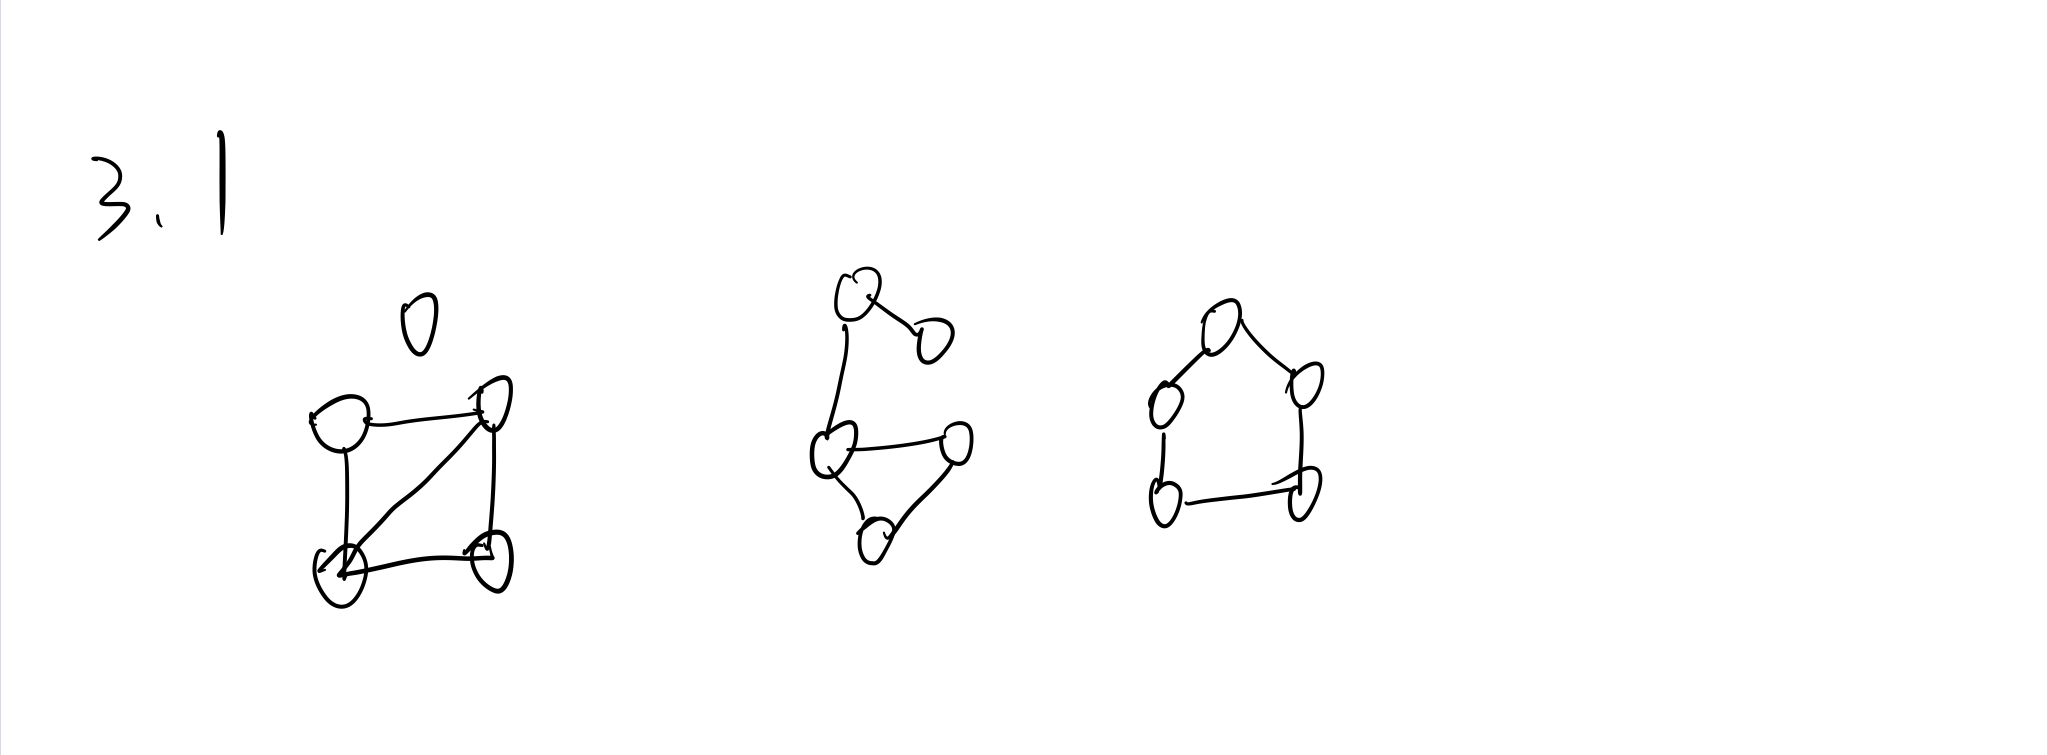
\includegraphics[width = 0.8\textwidth]{3.1.jpg}
\end{solution}
%%%%%%%%%%%%%%%

%%%%%%%%%%%%%%%
\begin{problem}[CZ 3.2]
\end{problem}

\begin{solution}
	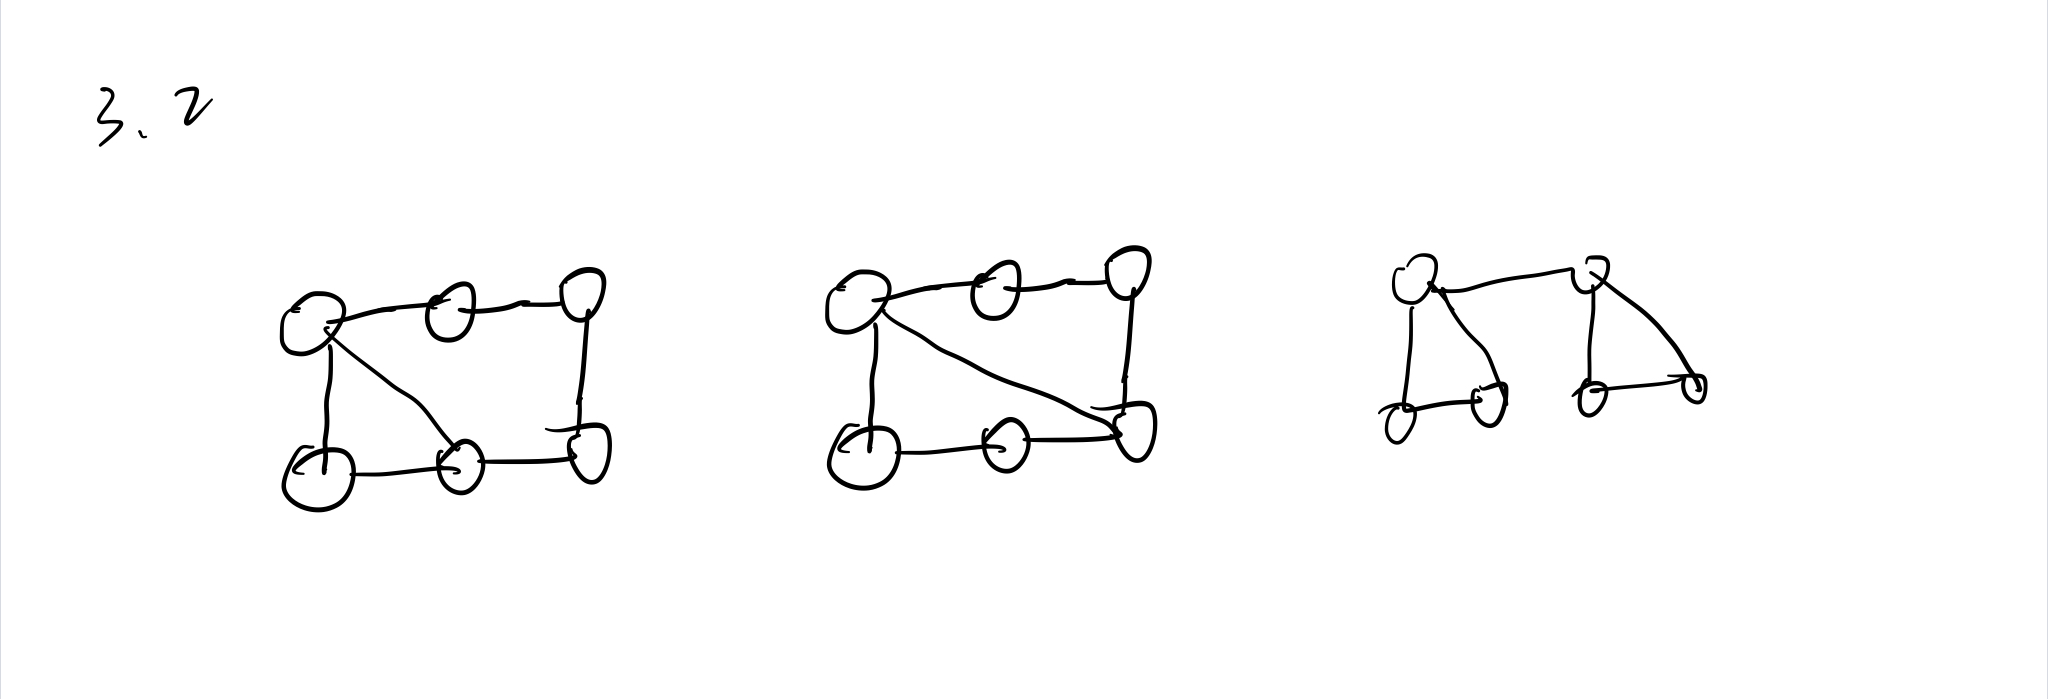
\includegraphics[width = 0.8\textwidth]{3.2.jpg}
\end{solution}
%%%%%%%%%%%%%%%

%%%%%%%%%%%%%%%%%%%%
\beginoptional

%%%%%%%%%%%%%%%
%\begin{problem}[TBD]
%\end{problem}
%
%\begin{solution}
%\end{solution}
%%%%%%%%%%%%%%%

%%%%%%%%%%%%%%%%%%%%
\beginot
%%%%%%%%%%%%%%%
\begin{ot}[图的应用-1]
	\begin{description}
		\item[\textbf{Tower of Hanoi}] 请尝利用Graph对汉诺塔问题进行建模,并指出在建模得到的图中,原先求解汉诺塔的问题,转换为图论中什么问题。
		\item[\textbf{Pagerank算法}]
			Pagerank如何对网络结构进行建模,以及大概的算法思想。

			参考资料:\href{https://en.m.wikipedia.org/wiki/PageRank}{https://en.m.wikipedia.org/wiki/PageRank}
	\end{description}
\end{ot}

% \begin{solution}
% \end{solution}
%%%%%%%%%%%%%%%

%%%%%%%%%%%%%%%
\begin{ot}[程序中的图]
	\begin{itemize}
		\item 简要介绍程序分析中常用各种图的基本概念。例如,调用图(Call Graph)、控制流图(Control-flow Graph)、程序依赖图(Program Dependence Graph)等。

		\item 参考资料:
		      \begin{itemize}
			      \item \href{https://en.m.wikipedia.org/wiki/Control-flow_graph}{https://en.m.wikipedia.org/wiki/Control-flow\_graph}
			      \item \href{https://en.m.wikipedia.org/wiki/Call_graph}{https://en.m.wikipedia.org/wiki/Call\_graph}
			      \item \href{https://dl.acm.org/doi/10.1145/24039.24041}{https://dl.acm.org/doi/10.1145/24039.24041}
		      \end{itemize}
	\end{itemize}

\end{ot}

% \begin{solution}
% \end{solution}
%%%%%%%%%%%%%%%


% \vspace{0.50cm}
%%%%%%%%%%%%%%%
% \begin{ot}[]
% 
%   \noindent 参考资料:
%   \begin{itemize}
%     \item 
%   \end{itemize}
% \end{ot}

% \begin{solution}
% \end{solution}
%%%%%%%%%%%%%%%

%%%%%%%%%%%%%%%%%%%%
% 如果没有需要订正的题目,可以把这部分删掉

% \begincorrection
%%%%%%%%%%%%%%%%%%%%

%%%%%%%%%%%%%%%%%%%%
% 如果没有反馈,可以把这部分删掉
\beginfb

% 你可以写
% ~\footnote{优先推荐 \href{problemoverflow.top}{ProblemOverflow}}:
% \begin{itemize}
%   \item 对课程及教师的建议与意见
%   \item 教材中不理解的内容
%   \item 希望深入了解的内容
%   \item $\cdots$
% \end{itemize}
%%%%%%%%%%%%%%%%%%%%
% \bibliography{2-5-solving-recurrence}
% \bibliographystyle{plainnat}
%%%%%%%%%%%%%%%%%%%%
\end{document}